\chapter{Memória}
De uma maneira geral, quando um processo é criado, sua imagem (ou parte dela) é armazenada em memória, onde a as instruções e os dados que estão sendo manipulados em um determinado instante são carregados na CPU. Os dados alterados são escritos em memória continuamente e os mais permanentes são armazenados em disco.

Um programa fonte apresenta instruções contendo endereços simbólicos, definidos pelo programador. Após o processo de compilação e montagem, o programa agora apresenta endereços relocáveis, construído em relação ao início do módulo onde são definidos. Após a \textit{linkagem}, o programa agora possui os endereços absolutos, único para o programa como um todo. Finalmente, com o \textit{loader}, quando o programa é carregado para a memória, os endereços físicos são efetivamente definidos. % TODO: ver se essa última sentença tá certa

\section{Gerenciamento}
O gerenciamento de memória é implementado pelo \textbf{gerente de memória}, responsável por definir e implementar a política de gerenciamento de memória do SO. Além disso, independente desta política, o gerente deve controlar a alocação das porções de memória aos processos, liberando-as quando estas não forem mais necessárias.






\subsection{Monitor Residente}
Em sistemas monoprogramados, a memória é geralmente dividida em duas áreas: uma para o usuário e outra para o sistema operacional.

Dessa forma, apenas um processo usuário está ativo por vez, pois a área de usuário é destinada a um processo apenas. Da mesma forma, a área do SO é ocupada por ele, o qual está sempre ativo.

Entretanto, é necessário um \textit{hardware} adicional, o qual vai impedir que processos de usuário invadão a área de memória do SO. É instaurada uma barreira, delimitando as áreas de memória, e a todo cálculo de endereço do processo usuário, o resultado é checado. A Figura \ref{fig:memory-fence} resume o processo.

\begin{figure}
  \centering
  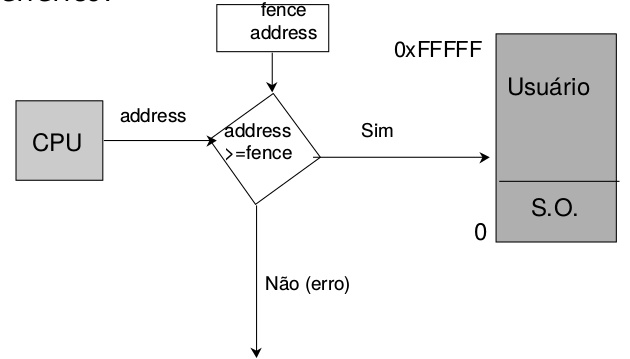
\includegraphics[width=0.65\textwidth]{memory-fence}
  \caption{O processo na CPU tentar acessar um endereço da memória. O \textit{hardware} checa se este endereço respeita o limite de área de memória do SO, liberando o acesso em caso positivo ou lançando um erro em caso negativo}
  \label{fig:memory-fence}
\end{figure}

Como \textbf{vantagens}, esta técnica tem implementação simples, pois só há um pequeno componente de proteção sendo usado. Além disso, os serviços do sistema operacional podem ser utilizados, como \textit{drivers}, interrupções, etc..

Como \textbf{desvantagem}, temos uma CPU sub-aproveitada, onde o sistema pode ser apenas mono-usuário e mono-tarefa






\subsection{Multiprogramação}
Multiprogramação é ofertada pela maioria dos computadores, onde vários processos coexistem na memória, havendo a necessidade da proteção de suas respectivas áreas de memória, evitando que um processo acesse a área de outro.

Logo, é lançado mão dos registradores de base e limite.




\subsection{Memória Virtual}



















\section{Paginação}
\subsection{Funcionamento}
\subsection{\textit{Page Fault}}
\subsection{Tabela de Páginas}
\subsection{Organização da Tabela de Páginas}
\subsection{Substituição de Páginas}
\subsection{Tratamento de \textit{Page Fault}}
